
\subsection{Librerías}%
\label{sub:librerias}

Si bien en muchos de los casos las librerías utilizadas en el desarrollo fueron configuradas por el componente~\textbf{Flex}  de \textbf{Symfony}, algunos paquetes
requirieron de una configuración más compleja y son los aquí listados.

\subsubsection{Instalación y Configuración de Sonata-User}%
\label{ssub:instalacion_y_configuración_de_sonata-user}

Esta librería integra el componente \textbf{FOSUser} de \textbf{Symfony} con \textbf{Sonata Admin} y agrega algunas características adicionales.




Para su instalación es necesario tener FOSUser instalado y configurado además de SonataAdmin y SonataEasyExtends\@.
Para este proceso se siguieron los pasos establecidos en la documentación de \textbf{Sonata-User}~\parencite{sonata-user}

\begin{figure}[H]
    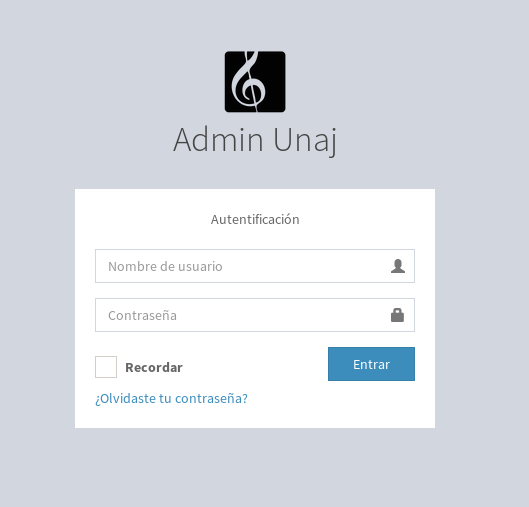
\includegraphics[width=1\linewidth]{image/adminLogin.png}
    \caption[Pantalla de login de Sonata-User]{Pantalla de login de Sonata-User.\newline \textbf{Fuente:} Elaboración propia, captura de pantalla de la aplicación web}
    \label{fig:image/adminLogin}
\end{figure}

\newpage
\textbf{Configuración básica:} Sonata User involucra varias librerías y elementos del sistema que deben ser configurados adecuadamente, estos son:

\begin{itemize}
    \item \textbf{Doctrine:} se debe definir el mapeo de entidades necesarias para el funcionamiento de la librería.
    \item \textbf{FOSUser:} se requiere especificar entidades y servicios para la administración de usuarios y grupos.
    \item \textbf{Security:} es necesario configurar la autenticación de usuarios y el control de acceso.
    \item \textbf{Routing:} se debe agregar información necesaria para la generación de rutas.
    \item \textbf{Sonata-User:} configuración que define el tipo de datos y las clases que definen la estructura de los datos de usuarios y grupos.
\end{itemize}



Como primer paso para la instalación y configuración de Sonata-User, se agregó la librería FOSUser y Sonata-User a través del gestor de paquetes Composer,
luego se comenzó con la configuración:

\paragraph{Sonata-User}~\newline

Se especificó a Sonata-User que los datos son administrados por un ORM.

\begin{lstlisting}[caption={archivo de configuración de sonata-user\\Fuente: \sonatainstallation.}]
#src/config/packages/sonata_user.yaml

sonata_user:
    manager_type: orm

\end{lstlisting}

\newpage \paragraph{FOSUser}~\newline

En cuanto a FOSUser se definió el driver de base de datos como ORM y el sistema de autenticación que utilizará\@. También se especificaron clases base
proporcionadas por Sonata-User, que serán utilizadas para la generación de las entidades finales de usuario y grupo\@. Por último, se definen los servicios
que administran estas entidades e información sobre el servicio de correo.

\begin{lstlisting}[caption={archivo de configuración de FOSUser\\ Fuente: \sonatainstallation.}]
#src/config/packages/fos_user.yaml

fos_user:
    db_driver: orm
    firewall_name: main
    user_class: Sonata\UserBundle\Entity\BaseUser
    group:
      group_class: Sonata\UserBundle\Entity\BaseGroup

      group_manager: sonata.user.orm.group_manager
    service:
      user_manager: sonata.user.orm.user_manager

    from_email:
        address: "test@domain.com"
        sender_name: "test@domain.com"

\end{lstlisting}

\newpage
\myparagraph{Doctrine}


La única configuración necesaria para el ORM es la definición explícita de cada una de las entidades mapeadas.
Doctrine cuenta con una característica llamada auto mapping, que permite cargar la configuración de entidades almacenadas bajo el directorio Entity/
de cada uno de los bundles.
Para la configuración de doctrine, cada entidad utilizada por Sonata-User y FOSUser debe estar definida en su archivo de configuración; pero dado que se
tiene habilitado la función de auto mapping y cada entidad está bajo un directorio de nombre “Entity” no es necesario agregar nada a la configuración existente.

\myparagraph{Routing}


Se agregaron las configuraciones de las rutas necesarias para ambas librerías.



\begin{lstlisting}[caption={archivo de configuración de rutas de FOSUser\\Fuente: \sonatainstallation.}]
#src/config/routes/fos_user.yaml

fos_user:
    resource: "@FOSUserBundle/Resources/config/routing/all.xml"
\end{lstlisting}

\newpage
\begin{lstlisting}[caption={archivo de configuración de rutas de sonata-user\\Fuente: \sonatainstallation.}]
#src/config/routes/sonata_user.yaml

sonata_user_admin_security:
    resource: '@SonataUserBundle/Resources/config/routing/admin_security.xml'
    prefix: /admin

sonata_user_admin_resetting:
    resource: '@SonataUserBundle/Resources/config/routing/admin_resetting.xml'
    prefix: /admin/resetting

\end{lstlisting}

\myparagraph{Security}

En cuanto a la configuración de seguridad, se definieron dos sistemas de autenticación (denominados firewall)\@. Uno se encargará de administrar la seguridad en
los usuarios admin y el otro en usuarios básicos.

\newpage
\begin{lstlisting}[caption={Firewall para el área admin del sistema.\\Fuente: \sonatainstallation.}]
#src/config/packages/security.yaml

# -> custom firewall for the admin area of the URL
        admin:
            pattern:            /admin(.*)
            context:            user
            form_login:
                provider:       fos_userbundle
                login_path:     /admin/login
                use_forward:    false
                check_path:     /admin/login_check
                failure_path:   null
                default_target_path: /admin/dashboard
            logout:
                path:           /admin/logout
                target:         /admin/login
            anonymous:          true
\end{lstlisting}

\newpage
\begin{lstlisting}[caption={Firewall para el área de registro y login de usuarios básicos.\\Fuente: \sonatainstallation.}]
#src/config/packages/security.yaml
        main:
            pattern:             .*
            context:             user
            form_login:
                provider:       fos_userbundle
                login_path:     /login
                use_forward:    false
                check_path:     /login_check
                failure_path:   null
            logout:             true
            anonymous:          true
\end{lstlisting}

\noindent
Además se especificó la jerarquía de roles y proveedor de usuarios:

\begin{lstlisting}[caption={Jerarquía de roles, tipo de encriptación y proveedor de usuarios\\Fuente: \sonatainstallation}]
    role_hierarchy:
        ROLE_ADMIN:       [ROLE_USER, ROLE_SONATA_ADMIN]
        ROLE_SUPER_ADMIN: [ROLE_ADMIN, ROLE_ALLOWED_TO_SWITCH]
        SONATA:
            - ROLE_SONATA_PAGE_ADMIN_PAGE_EDIT

    providers:
        fos_userbundle:
            id: fos_user.user_provider.username

    encoders:
        FOS\UserBundle\Model\UserInterface: bcrypt
\end{lstlisting}

\newpage
Por último, se define el control de acceso de manera que se pueda ingresar anónimamente a cada página de registro, inicio de sesión, reinicio de contraseña,
etc.
También se especifica qué roles tienen permitido ingresar a la parte de administración del sistema.

\begin{figure}[H]
    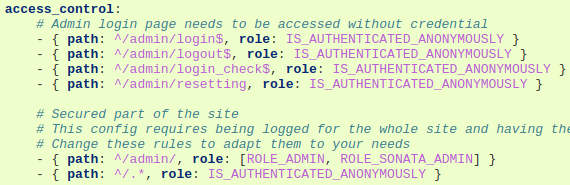
\includegraphics[width=1\linewidth]{image/acl.png}
    \caption[Control de acceso]{Control de acceso.\newline \textbf{Fuente:} Recuperado de https://sonata-project.org/bundles/user/master/doc/reference/installation.html}
    \label{fig:image/acl}
\end{figure}

\myparagraph{Generación de entidades finales}

A partir de esta configuración se generaron las entidades de usuario y grupo mediante el comando:

\begin{lstlisting}
bin/console sonata:easy-extends:generate SonataUserBundle --dest=src --namespace_prefix=App
\end{lstlisting}


Esto da como resultado un directorio en \textbf{Application\textbackslash Sonata\textbackslash UserBundle} el cual contiene las entidades a utilizar por las librerías.
Por último, se configuró Sonata-User y FOSUser para que utilicen las nuevas entidades:

\newpage
\begin{lstlisting}[caption={Archivo de configuración de Sonata-User.\\Fuente: \sonatainstallation}]
#src/config/packages/sonata_user.yaml

sonata_user:
  manager_type: orm
  class:
        user: App\Application\Sonata\UserBundle\Entity\User
        group: App\Application\Sonata\UserBundle\Entity\Group

\end{lstlisting}

\begin{lstlisting}[caption=Archivo de configuración de FOSUser.\\Fuente: \sonatainstallation]
#src/config/packages/fos_user.yaml

fos_user:
    db_driver: orm # other valid values are 'mongodb' and 'couchdb'
    firewall_name: main
    user_class: App\Application\Sonata\UserBundle\Entity\User
    group:
      group_class:   App\Application\Sonata\UserBundle\Entity\Group
      group_manager: sonata.user.orm.group_manager
    service:
      user_manager: sonata.user.orm.user_manager

    from_email:
        address: "test@domain.com"
        sender_name: "test@domain.com"

\end{lstlisting}

\newpage
\subsubsection{API-Platform}%
\label{ssub:api_platform}

Para la instalación de esta librería sólo es necesario agregarla a través de \textbf{Composer} y Flex se hace cargo de la configuración\@. Luego de realizado
esto, se configuró las entidades a exponer, que en este caso serían todas las entidades que representan datos en el sistema.


API-Platform permite definir las entidades a utilizar durante el proceso de serialización mediante anotaciones o archivos de configuración. Por defecto,
este componente serializa todos los campos y todas aquellas funciones que retornen algún valor\@. Probablemente se tengan entidades con funciones o datos
que no se quieran exponer a los usuarios. Además, se pueden encontrar referencias circulares entre algunas entidades, que fue lo que sucedió entre miembros
y roles de proyecto (un miembro tiene un rol, y un rol tiene muchos miembros)\@.  Por este motivo, se decidió configurar la información que es expuesta a
través de estas entidades.

\newpage
\myparagraph{El proceso de serialización}


La serialización es el proceso de convertir estructuras de datos u objetos en un formato que puede ser almacenado (por ejemplo, en un archivo o búfer de memoria)
o transmitido (por ejemplo, a través una conexión de red) y reconstruido luego (posiblemente en un entorno diferente).~\parencite{serialization}

\begin{figure}[H]
    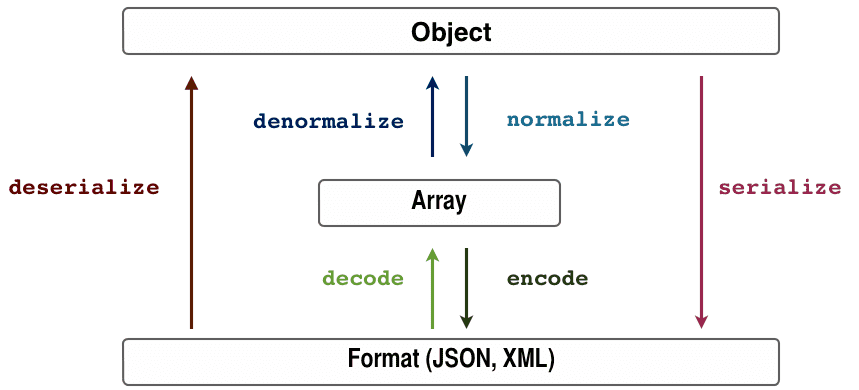
\includegraphics[width=1\linewidth]{image/serializationWorkflow.png}
    \caption[El proceso de serialización]{El proceso de serialización.\newline \textbf{Fuente:} Recuperado de~https://api-platform.com/docs/core/serialization/}
    \label{fig:image/serializationWorkflow}
\end{figure}

En \textbf{Symfony} esto es logrado a través del componente \textbf{Serializer}. El proceso en sí, sigue el esquema presentado en la figura
\ref{fig:image/serializationWorkflow}\@.
Para la conversión primero se convierte el objeto en un \textit{array} (proceso denominado
normalización) y luego se convierte al formato específico que se necesite (a este proceso se lo llama codificación).

API-Platform permite modificar la información que se expone a los usuarios mediante grupos de \textit{serialización} y \textit{deserialización}\@. A través del uso de anotaciones
en cada propiedad de la entidad se puede definir si agregar la propiedad al proceso de normalización o no dependiendo de la acción que se esté realizando.
Si se desean funciones más complejas, es posible definir \textit{normalizadores} y \textit{codificadores} personalizados o decorar \textit{normalizadores} existentes.
~\parencite{api-platform-serialization}

\myparagraph{Modificación del proceso de serialización}

Mediante anotaciones se agregó cada propiedad relevante a cada acción en particular y se omitieron aquellas propiedades o funciones que no necesitan estar
presentes o que no se desean exponer a los usuarios.

Al definir un grupo de serialización se logra que, al agregar una propiedad al contexto de normalización, sólo se serialice las propiedades pertenecientes
al grupo en cuestión. Esto significa, que si se agrega una relación al contexto de normalización, se serializarán los campos de la entidad relacionada
que pertenezcan a dicho grupo.


\subsubsection{Guzzle y EightPointsGuzzle}%
\label{ssub:guzzle}

Guzzle es una librería que facilita la interacción con servicios web, al proveer métodos simples para realizar solicitudes \textbf{HTTP}\@. Su funcionamiento consiste en la creación
de un objeto llamado \textbf{cliente}, el cual provee acceso al servicio web a utilizar.


Eightpoints integra Guzzle con Symfony y permite definir un cliente como servicio de manera que sea posible utilizarlo en cualquier parte de la aplicación.


Se utilizaron estas dos librarías para configurar los servicios web a integrar con RUDA. Su configuración requiere de la ruta base de la API para funcionar y es posible definir
diversas opciones como headers y autenticación.


Se definió un cliente Guzzle para el servicio web de mapuche definiendo su ruta base, método de autenticación y headers. Como autenticación se utilizó HTTP digest y se definieron
 headers que definen el formato a utilizar como \textbf{json}.
